\documentclass[tikz,border=12pt]{standalone}
\usepackage[T1]{fontenc}
\usepackage{mathpazo}
\usepackage{amsmath,amssymb}
\usetikzlibrary{arrows.meta, calc}

\definecolor{stblue}{HTML}{7B97AD}
\definecolor{rwgold}{HTML}{B8995E}
\definecolor{sage}{HTML}{7A9A7E}
\definecolor{dkbrown}{HTML}{3D3530}
\definecolor{wmgray}{HTML}{7B7067}
\definecolor{cream}{HTML}{F9F6F0}
\definecolor{border}{HTML}{D4C9B8}
\definecolor{terracotta}{HTML}{C47A6A}
\definecolor{lavender}{HTML}{907EA0}

\begin{document}
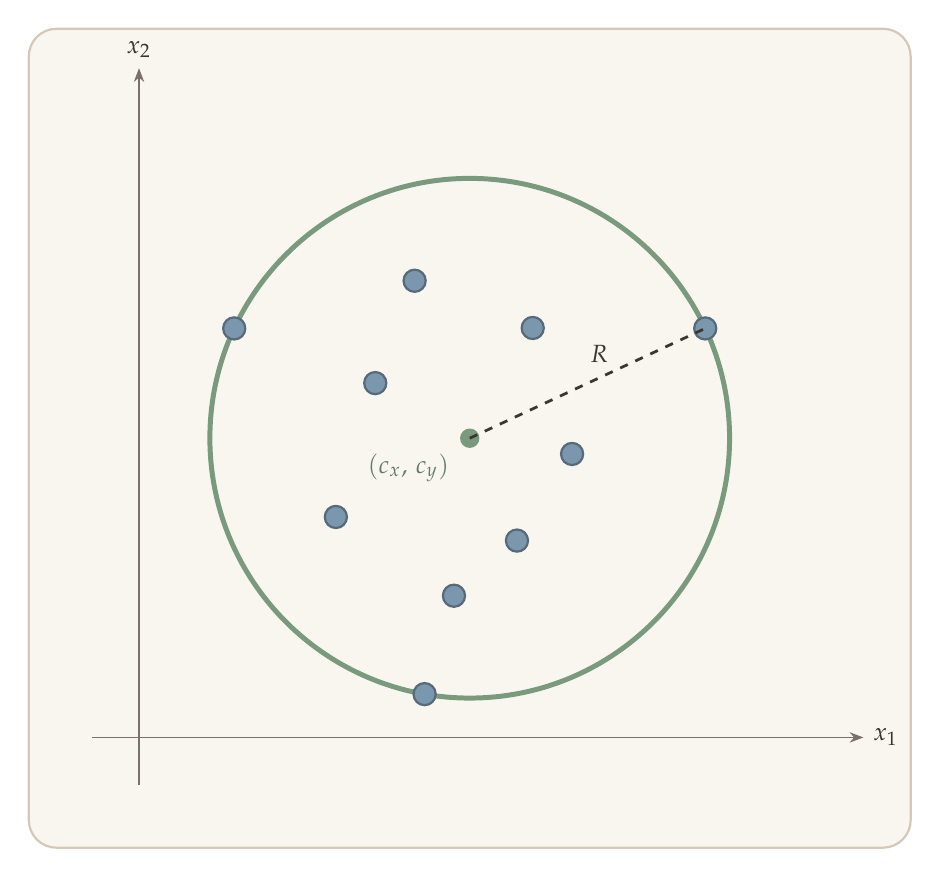
\begin{tikzpicture}[
  >={Stealth[length=3.5mm, width=2.5mm]},
  axis/.style={-{Stealth[length=5pt]}, wmgray, line width=0.6pt},
  lbl/.style={dkbrown, font=\small},
]

% ══════════════════════════════════════════════════════
% Geometry setup
% ══════════════════════════════════════════════════════
% Circle center and radius
\pgfmathsetmacro{\cx}{4.2}
\pgfmathsetmacro{\cy}{3.8}
\pgfmathsetmacro{\R}{3.3}

% ══════════════════════════════════════════════════════
% Background
% ══════════════════════════════════════════════════════
\fill[cream, rounded corners=10pt] (-1.4,-1.4) rectangle (9.8,9.0);
\draw[border, line width=0.8pt, rounded corners=10pt]
  (-1.4,-1.4) rectangle (9.8,9.0);

% ══════════════════════════════════════════════════════
% Axes
% ══════════════════════════════════════════════════════
\draw[axis] (-0.6,0) -- (9.2,0) node[right, lbl] {$x_1$};
\draw[axis] (0,-0.6) -- (0,8.5) node[above, lbl] {$x_2$};

% ══════════════════════════════════════════════════════
% Smallest enclosing circle
% ══════════════════════════════════════════════════════
\draw[sage, line width=1.8pt] (\cx, \cy) circle (\R);

% ══════════════════════════════════════════════════════
% Center point
% ══════════════════════════════════════════════════════
\fill[sage] (\cx, \cy) circle (3.5pt);

% Center label
\node[sage!80!black, font=\small, anchor=north east, xshift=-4pt, yshift=-2pt]
  at (\cx, \cy) {$(c_x,\, c_y)$};

% ══════════════════════════════════════════════════════
% Points on the circle boundary (these determine the solution)
% ══════════════════════════════════════════════════════
% Point B1: angle 25 degrees
\pgfmathsetmacro{\bAx}{\cx + \R*cos(25)}
\pgfmathsetmacro{\bAy}{\cy + \R*sin(25)}
% Point B2: angle 155 degrees
\pgfmathsetmacro{\bBx}{\cx + \R*cos(155)}
\pgfmathsetmacro{\bBy}{\cy + \R*sin(155)}
% Point B3: angle 260 degrees
\pgfmathsetmacro{\bCx}{\cx + \R*cos(260)}
\pgfmathsetmacro{\bCy}{\cy + \R*sin(260)}

\foreach \px/\py in {\bAx/\bAy, \bBx/\bBy, \bCx/\bCy}{
  \fill[stblue] (\px, \py) circle (4pt);
  \draw[stblue!70!black, line width=0.8pt] (\px, \py) circle (4pt);
}

% ══════════════════════════════════════════════════════
% Interior points (strictly inside the circle)
% ══════════════════════════════════════════════════════
\foreach \px/\py in {%
  3.0/4.5,%
  5.0/5.2,%
  4.8/2.5,%
  2.5/2.8,%
  3.5/5.8,%
  5.5/3.6,%
  4.0/1.8%
}{
  \fill[stblue] (\px, \py) circle (4pt);
  \draw[stblue!70!black, line width=0.8pt] (\px, \py) circle (4pt);
}

% ══════════════════════════════════════════════════════
% Radius line from center to boundary point B1
% ══════════════════════════════════════════════════════
\draw[dkbrown, line width=1.0pt, dashed]
  (\cx, \cy) -- (\bAx, \bAy);

% R label along the radius line
\node[dkbrown, font=\small, anchor=south, yshift=2pt]
  at ($(\cx, \cy)!0.55!(\bAx, \bAy)$) {$R$};

\end{tikzpicture}
\end{document}
